% document formatting
\documentclass[10pt]{article}
\usepackage[utf8]{inputenc}
\usepackage[left=1in,right=1in,top=1in,bottom=1in]{geometry}
\usepackage[T1]{fontenc}
\usepackage{xcolor}

% math symbols, etc.
\usepackage{amsmath, amsfonts, amssymb, amsthm}

% lists
\usepackage{enumerate}

% images
\usepackage{graphicx} % for images

% code blocks
\usepackage{minted, listings} 

% verbatim greek
\usepackage{alphabeta}

\graphicspath{{./assets/images}}

\newcommand{\solution}{\textbf{Solution:}} 
\newcommand{\example}{\textbf{Example: }}

\title{EC ENGR 102 Week 4}

\author{Aidan Jan}
\date{\today}

\begin{document}
\maketitle

\subsection*{Using Commutativity to Show System Stability}
\begin{itemize}
    \item BIBO Stability: if $|x(t)| \leq M_x < \infty$ and $y(t) = H(x(t))$, then $H$ is BIBO stable if $|y(t)| \leq M_y < \infty$.
    \item Commutativity states:
    \begin{align*}
        |y(t)| &= \left|\int_{-\infty}^\infty x(\tau) h(t - \tau) \text{d}\tau\right|\\
        &= \left|\int_{-\infty}^\infty h(\tau) x(t - \tau) \text{d}\tau \right|
        &\leq \int_{-\infty}^\infty |h(\tau)| \cdot |x(t - \tau| \text{d}\tau)\\
        &\leq \int_{-\infty}^\infty |h(\tau) \cdot M_x \text{ d}t\\
        &= M_x \cdot \int_{-\infty}^\infty |h(\tau)| \text{ d}\tau\\
        &\leq M_y
    \end{align*}
    Therefore, $H$ is stable.
    \[\text{If } \int_{-\infty}^\infty |h(\tau)| \text{ d}\tau \leq M_h < \infty \Rightarrow \text{ H is BIBO stable.}\]

    
\end{itemize}

\subsection*{Proof of Associativity}
Show that:
\[(f * (g * h))(t) = ((f * g) * h)(t)\]
First, note that
\[y(t - \alpha) = \int_{-\infty}^\infty x(\tau) h(t - \alpha - \tau) \text{d}\tau\]
as per the definition of the convolution.\\\\
Starting with the left-hand side:
\begin{align*}
f * (g * h)(t) &= \int_{-\infty}^\infty f(\tau_1) \cdot (g * h)(t - \tau_1) \text{d}\tau_1\\
&= \int_{-\infty}^\infty f(\tau_1) \cdot \int_{-\infty}^\infty g(\tau_2) h(t - \tau_1 - \tau_2) \text{ d}\tau_2 \text{ d}\tau_1\\
\intertext{Let $\tau_2 = \tau_3 - \tau_1$.  Therefore, $\tau_3 = \tau_1 + \tau_2$ and $\text{d}\tau_2 = \text{d}\tau_3$}\\
&= \int_{-\infty}^\infty f(\tau_1) \cdot \int_{-\infty}^\infty g(\tau_3 - \tau_1) \cdot h(t - \tau_3) \text{ d} \tau_3 \text{ d}\tau_1\\
\intertext{Now, we can change the order of integration.}\\
&= \int_{-\infty}^\infty h(t - \tau_3) \cdot \int_{-\infty}^\infty f(\tau_1) \cdot g(\tau_3 - \tau_1) \text{ d} \tau_1 \text{ d} \tau_3\\
&= \int_{-\infty}^\infty h(t - \tau_3) (f * g) (\tau_3) \text{ d}\tau_3\\
&= \int_{-\infty}^\infty (f * g)(\tau_3) h(t - \tau_3) \text{ d}\tau_3\\
&= (f * g) * h
\end{align*}

\subsection*{Proof of Distributivity}
Show that:
\[f * (g + h) = f * g + f * h\]
To prove this, we write out the definition of convolution:
\begin{align*}
    (f * (g + h))(t) &= \int_{-\infty}^\infty f(\tau)[g(t - \tau) + h(t - \tau)] \text{d}\tau\\
    &= \int_{-\infty}^\infty f(\tau) g(t - \tau) \text{d}\tau + \int_{-\infty}^\infty f(\tau) h(t - \tau) \text{d}\tau\\
    &= (f * g)(t) + (f * h)(t)
\end{align*}

\subsection*{Identity Element of Convolution}
Here, we have something that looks like an "algebra of signals," with addition like in ordinary algebra, and multiplication is replaced by convolution.  In standard algebra, the multiplicative identity is 1.  In signals, the convolution identity is the Dirac delta function, $\delta(t)$.\\\\
In particular, note that:
\[\boxed{x(t) * \delta(t) = x(t)}\]
because
\begin{align*}
    x(t) * \delta(t) &= \int_{-\infty}^\infty x(\tau) \delta(t - \tau) \text{d} \tau\\
    &= \int_{-\infty}^\infty \delta(\tau) x(t - \tau) \text{d}\tau\\
    &= \int_{-\infty}^\infty \delta(\tau)x(t) \text{d}\tau\\
    &= x(t)\int_{-\infty}^\infty \delta(\tau) \text{d}\tau\\
    &= x(t)
\end{align*}
\subsection*{Delay via Convolution}
Convolution with the impulse can also be used to delay signals, i.e.,
\[\boxed{x(t) * \delta(t - t_d) = x(t - t_d)}\]
To prove this, note that:
\[x(t) * \delta(t - t_d) = \int_{-\infty}^\infty x(\tau) \delta(t - t_d - \tau)\text{d}\tau\]
i.e., $x(\tau)$ is being multiplied by an impulse that occurs at $\tau = t - t_d$.  From what we know about convolution, this extracts out the value of $x(\tau)$ at $t - t_d$.\\
So,
\begin{align*}
    x(t) * \delta(t - t_d) &= \int_{-\infty}^\infty x(\tau) \delta(t - t_d - \tau) \text{d}\tau\\
    &= \int_{-\infty}^\infty x(t - t_d) \delta(t - t_d - \tau) \text{d}\tau\\
    &= x(t - t_d) \int_{-\infty}^\infty \delta(t - t_d - \tau) \text{d}\tau\\
    &= x(t - t_d)
\end{align*}

\subsection*{Integration Through Convolution}
Convolution can be used to implement integration.   In particular, to integrate a signla $x$ from $-\infty$ to $t$, we integrate it with a unit step.
\begin{align*}
    x(t) * u(t) &= \int_{-\infty}^\infty x(\tau) u(t - \tau) \text{d}\tau\\
    &= \int_{-\infty}^t x(\tau) \text{d}\tau
\end{align*}
where we used the fact that $u(t - \tau)$ is zero for when $\tau > t$.

\subsection*{Additional Properties of Convolution}
Given these properties of convolution, there are now a few properties we cah derive regarding convolution.
\begin{itemize}
    \item \textbf{Linearity:} Convolution is \textbf{linear}, since for all signals $x_1, x_2$ and all $\alpha, \beta \in \mathbb{R}$.
    \[h * (\alpha x_1 + \beta x_2) = \alpha(h * x_1) + \beta(h * x_2)\]
    \item \textbf{Time-invariance:} if $y(t) = x(t) * h(t)$, then if we delay the input by $T$, i.e., the new input is $x(t - T)$, then the output is $y(t - T)$.
    \item \textbf{Cascade (composition):} Due to the associativity of convolution, the cascade connection of two convolutions systems, $y = (x * f) * g$ is equivalent to a single system $y = x * h$, where $h = f * g$.  That is, the following two block diagrams are equivalent:
    \begin{center}
        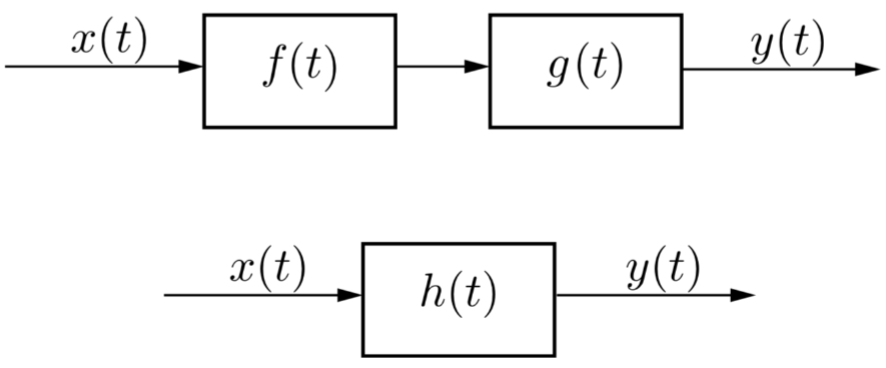
\includegraphics[scale=0.7]{W4_1.png}
    \end{center}
    \item \textbf{Swapping (composition II):} If $y = (x * f) * g$, then due to the commutivity of convolution, this is equivalent to $y = (x * g) * f$.  This means that you can swap the order of convolutions, as illustrated in the block diagram below:
    \begin{center}
        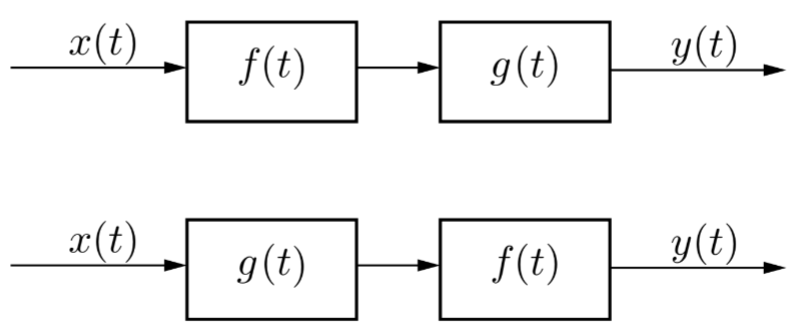
\includegraphics[scale=0.7]{W4_2.png}
    \end{center}
    Many operations can be written as convolutions (integration, delays, differentiation, etc.) and these operations all commute.
\end{itemize}

\subsubsection*{Question: How are the Impulse and Step Response related?}
\begin{center}
    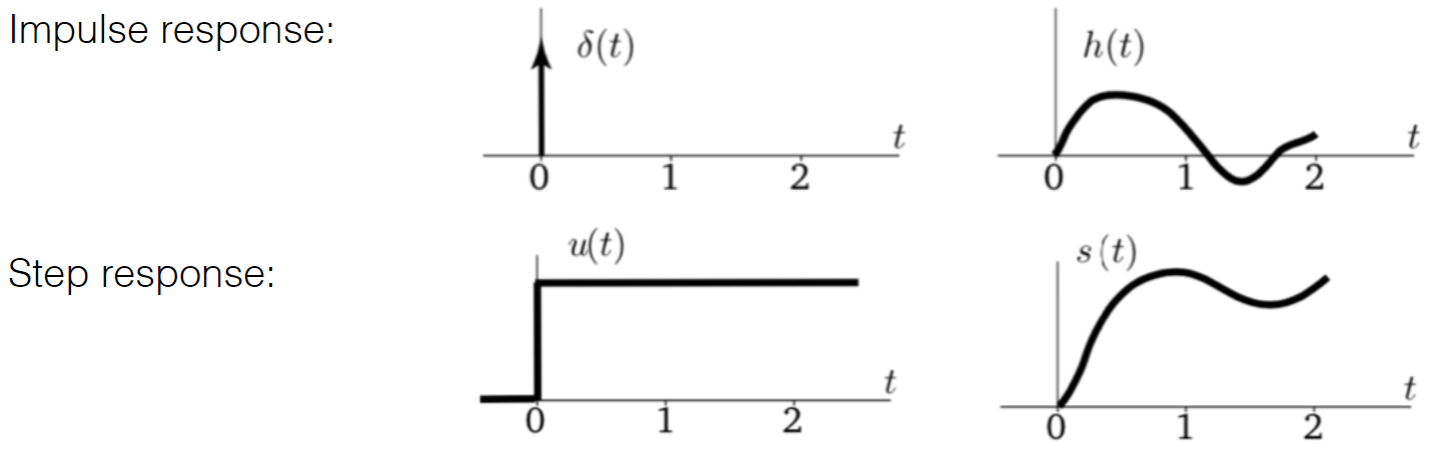
\includegraphics[scale=0.5]{W4_3.png}
\end{center}
It turns out that the integral of the impulse response is the step response!  (This makes sense since the integral of the Dirac delta function is the unit step.)\\
\hrulefill\\
Due to commutivity, we can now find the impulse response by differentiating the step response, i.e.,
\[h(t) = \frac{\text{d}s(t)}{\text{d}t}\]
This is illustrated below.
\begin{center}
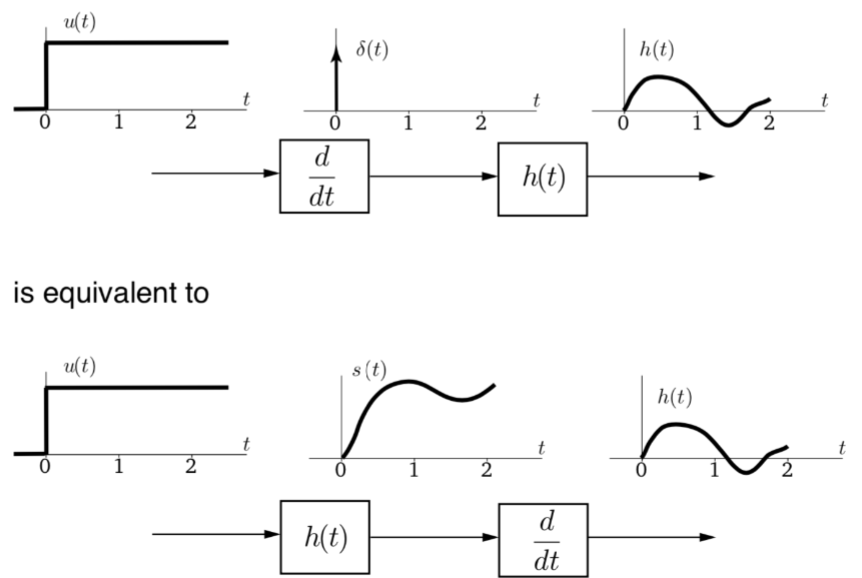
\includegraphics[scale=0.5]{W4_4.png}
\end{center}

\subsection*{Recap on LTI Systems and Convolution}
\begin{enumerate}
    \item \textbf{Any LTI system can be characterized by an impulse response.}\\\\
    This means that if I know the impulse response, I can calculate the output of the system for any given input.\\\\
    \textit{Example application:} consider playing baseball.  Swinging the bat, and making contact with a ball is like a brief impulse (force) applied from the bat to the ball.  How the ball flies through the air is an example of an impulse response.\\\\
    \textit{Example application:} consider a stringed instrument.  When I pluck the string, it begins to vibrate.  Its vibration is an impulse response.\\\\
    \textbf{Step responses} are more common.\\\\
    \textit{Example application:} I step on the gas pedal of my car.  The car's response is an example of a step response, and it looks different depending on the car (e.g., an EV vs. a gas car).\\\\
    \textit{Example application:} I flip a switch, which turns on the power to a circuit.  How the circuit acts when I flip the switch is its step response.
    \item To calculate the impulse response, we input an impulse to the system and measure the output.
    \item After we know the impulse response, we can caltulate the output for any given input via the convolution integral.
    \[\boxed{y(t) = \int_{-\infty}^\infty x(\tau) h(t - \tau) \text{d}\tau}\]
    \item This operation has several properties.
    \begin{itemize}
        \item Commutativity
        \item Associativity
        \item Distributivity
        \item Identity Element
        \item Delay
        \item LTI
        \item Composition
    \end{itemize}
\end{enumerate}

\subsubsection*{Other Examples of Swapping:}
\begin{itemize}
    \item Say I wanted to edit a piece of music by making the treble quieter.  After this, I still wasn't happy with the recording and wanted to make the bass louder.  These happen to both be LTI operations and can be done in either order.
    \item Say I have an LTI circuit, and I want to know what happens when it receives a jolt of brief power (e.g., from a temporary power surge).  I can estimate this by giving it constant power input (a step), and then differentiating the circuit's response to the step.
\end{itemize}

\section*{Fourier Series}
\begin{itemize}
    \item Any periodic signal can be expressed as a sum of sinusoids. (complex exponentials).
    \item The sinusoids that make up the signal are called the Fourier Series.
    \item In terms of math,
    \[x(t) = x_1(t) + x_2(t) + \dots\]
    where each $x_i(t)$ is written in the form $e^{j\omega t} = \cos(\omega t) + j \cdot \sin(\omega t)$
\end{itemize}

\subsection*{Bottom Line}
If $f(t)$ is a well-behaved (continuous) periodic signal with period $T_0$, then $f(t)$ can be written as a Fourier series
\[\boxed{f(t) = \sum_{k = -\infty}^\infty c_k e^{jk\omega_0 t}}\]
where $\omega_0 = \frac{2\pi}{T_0}$ and
\[\boxed{c_k = \frac{1}{T_0} \int_\tau^{\tau + T_0} f(t) e^{-jk\omega_o t}\text{d}t}\]
for all integers $k$.  The $c_k$ are called the \textit{Fourier coefficients} of $f(t)$.\\\\
Here, $f(t)$ is the \textit{weighted average} of complex exponentials (which are simply complex sines and cosines).

\subsection*{Implications for LTI Systems}
We know that for a linear system, if $x(t) = x_1(t) + x_2(t) + \cdots + x_n(t)$, then
\begin{align*}
    y(t) &= h(t) * x(t)\\
    &= h(t) * (x_1(t) + x_2(t) + \cdots + x_n(t))\\
    &= h(t) * x_1(t) + h(t) * x_2(t) + \dots h(t) * x_n(t)
\end{align*}
What this tells us is that if we can decompose our signal, $x(t)$, into its components, we can calculate the system output by considering each of these components in isolation.  After this, we sum the outputs of these components together.\\\\
Fourier's idea, in 1807, was to decompose $x(t)$ using one of the most basic signals we know of: sines and cosines.

\subsection*{Eigenfunctions of LTI systems}
\begin{itemize}
    \item $x(t)$ is an \textit{eigenfunction} of a system, if, when inputting $x(t)$ to the system, the output is simply a scaled version of $x(t)$, i.e., $y(t) = ax(t)$ where $a$ is a constant (called an eigenvalue).  Note that $a$ may be a complex constant.
    \item \textbf{Complex exponentials are eigenfunctions of LTI systems}
    \begin{itemize}
        \item When a complex exponential (eigenfunction) is input into an LTI function, the resulting function is \textbf{always} the same function, possibly with amplitude and phase angle changes.  The frequency remains the same.
    \end{itemize}
\end{itemize}

\pagebreak
\subsection*{Deriving the Eigenfunctions of LTI Systems}
Consider an LTI system with impulse response $h(t)$.  If the input is a complex exponential, i.e., $e^{st}$ where $s = \sigma + j\omega$, then
\[y(t) = \int_{-\infty}^\infty h(\tau) e^{s(t - \tau)}\text{d}\tau\]
We can start by splitting up the exponent.

\begin{align*}
    y(t) &= \int_{-\infty}^\infty h(t) e^{st} \cdot e^{-s\tau} \text{d}\tau\\
    &= e^{st} \cdot \int_{-\infty}^\infty h(\tau) e^{-s\tau} \text{d}\tau\\
    \intertext{Notice that the integral is now a function of $s$.  There are no other variables present in there (also not dependent on $t$).  Therefore, we can write it as such.}
    &= H(s) \cdot e^{st}
\end{align*}
where $H(s) = \int_{-\infty}^\infty h(\tau) e^{-s\tau} \text{d}\tau$, called the "Transfer Function".

\[e^{st} \:\longrightarrow\:\boxed{\text{LTI System} * h(t)} \longrightarrow \: a\cdot e^{st}\]
where $a = H(s)$

\subsection*{Proving that LTI functions on a Fourier series returns a Fourier series}
Say $x(t) = \sum_{k = -\infty}^\infty c_k \cdot e^{jk\omega_0 t}$.  $x(t)$ is then a fourier series and is periodic.\\\\
Take one complex exponential, $k = 1 \Rightarrow x_1(t) = c_1 \cdot e^{j\omega_0 t}$\\\\
In this case,
\[x_1(t) \longrightarrow \boxed{\text{LTI}}\longrightarrow y_1(t) = H(j\omega_0) \cdot c_1 \cdot e^{j \omega_0 t}\]
Now, we take another complex exponential, $k = 2 \Rightarrow x_2(t) = c_2 e^{j \cdot 2\omega_0 t}$\\\\
Now, we get
\[x_2(t) \longrightarrow\boxed{\text{LTI}}\longrightarrow y_2(t) = H(j\omega_2) \cdot c_2 \cdot e^{j \cdot 2\omega_0 t}\]
And we continue doing this for everything in the sum.\\\\
By the linearity property $x_1(t) + x_2(t) \rightarrow\boxed{\text{LTI}}\rightarrow y_1(t) + y_2(t)$, so
\begin{align*}
    x(t) &= \sum_{k = -\infty}^\infty c_k e^{jk\omega_0 t}\\
    \Rightarrow y(t) &= \sum_{k = -\infty}^\infty H(jk\omega_0) \cdot c_k e^{jk\omega_0 t}\\
    &= \sum_{k = -\infty}^\infty c_k e^{jk\omega_0}
\end{align*}
Essentially, every fourier series can be broken down into the sum of many complex sinusoidals, each of which passing through the LTI system would become another complex sinusoidal.  By adding them up, we receive another fourier series.  Therefore, a fourier series passed into an LTI would return another fourier series.

\subsection*{Fourier Series Example}
Let's start simple.  Consider the sinusoid:
\[f(t) = A \cos(\omega_0 t + \theta)\]
Converting to exponential form, we get:
\begin{align*}
    f(t) &= \frac{A}{2} e^{-j(\omega_0 t + \theta)} + \frac{A}{2} e^{j(\omega_0 t + \theta)}\\
    &= \frac{A}{2} e^{-j^\theta} \cdot e^{-j \omega_0 t} + \frac{A}{2} e^{j^\theta} \cdot e^{j\omega_0 t}
\end{align*} 
\begin{itemize}
    \item Notice the first term, written in form $c_k \cdot e^{-j\omega t}$, would be $c_{-1}$, and the second term would be $c_1$.
    \item Both terms have amplitude $\frac{A}{2}$.
    \item The first term has a phase of $-\omega_0$ while the second has $\omega_0$.
    \item We can plot these on the spectrum. (remember that every signal can be defined by the spectrums!)
\end{itemize}

\subsection*{Using Spectrum to Find Structure}
Suppose we were given the following signal:
\begin{center}
    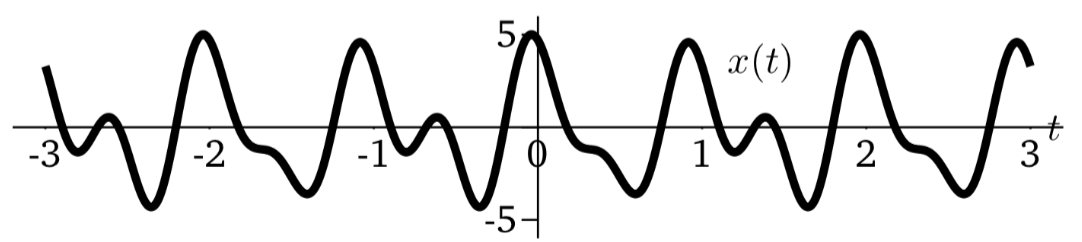
\includegraphics[scale=0.7]{W4_5.png} 
\end{center}
This signal is very simple, but it's hard to recover what $x(t)$ is.  However, if given the spectrum:
\begin{center}
    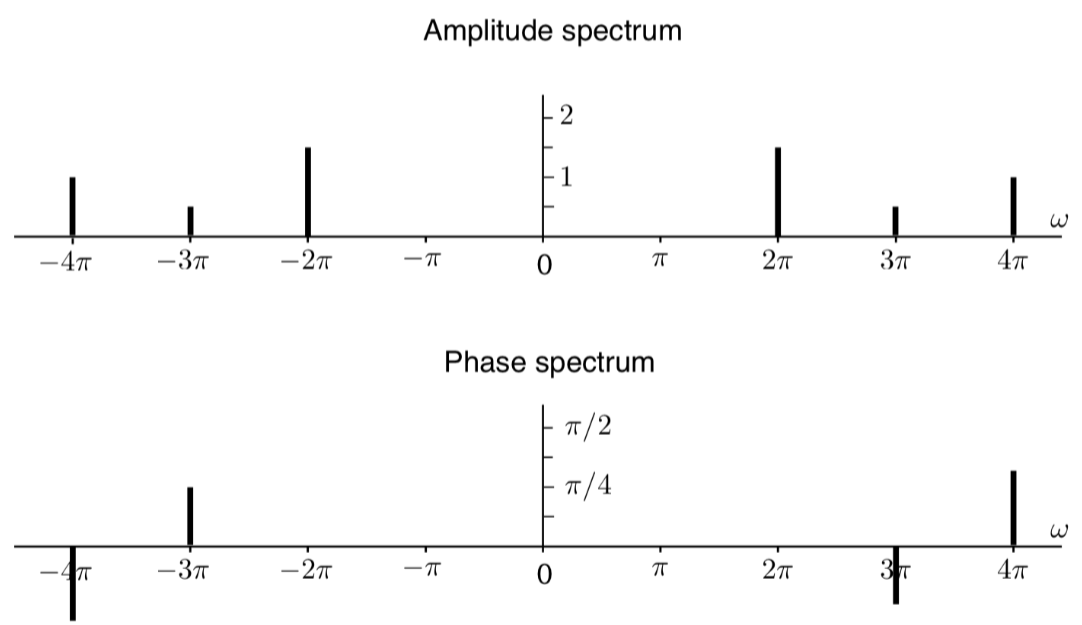
\includegraphics[scale=0.7]{W4_6.png}
\end{center}
From the spectrum, we can read off that this signal is composed of sinusoids at three different frequencies ($2\pi, 3\pi, 4\pi$) with amplitudes given by the amplitude spectrum and phases given by the phase spectrum.\\\\
We get:
\begin{itemize}
    \item Signal 1: Frequency $2\pi$, Amplitude $3$, Phase $0$.
    \item Signal 2: Frequency $3\pi$, Amplitude $1$, Phase $\pi/4$.
    \item Signal 3: Frequency $4\pi$, Amplitude $2$, Phase $-\pi/3$.
    \begin{align*}
        x(t) &= 1.5 \cdot e^{j_0} \cdot e^{-j \cdot 2\pi t} + 1.5 \cdot e^{j_0} \cdot e^{j \cdot 2\pi t}\\
        &\hspace{0.5cm}+ 0.5 \cdot e^{j\pi/4} \cdot e^{-j\cdot 3\pi t} + 0.5 \cdot e^{-j\pi/4} \cdot e^{j\cdot 3\pi t}\\
        &\hspace{0.5cm}+ 1 \cdot e^{-j\pi/3} \cdot e^{-j \cdot 4\pi t} + 1 \cdot e^{j\pi/3} \cdot e^{j \cdot 4\pi t}\\
        &= 3\cos(2\pi t) + \cos (3\pi t - \pi / 4) + 2\cos(4\pi t + \pi/3)
    \end{align*}
    
\end{itemize}

\subsection*{Deriving the Fourier Series Coefficients}
How do we find the $c_k$?  Remember that $c_k$ is some constant, that is a complex value.\\\\
Our derivation is as follows:
\begin{itemize}
    \item First, we \textit{assume} that the signal $f(t)$ can be written as a sum of complex exponentials that are scaled by coefficients $c_k$.
    \item Given this assumption, we find if there are $c_k$ such that we can represent $f(t)$ in this way.
\end{itemize}

\subsubsection*{A Preliminary result on integrating complex exponentials}
Before proceeding, we're going to introduce a handy trick that will simplify our derivation.  Let $T_0 = 2\pi / \omega_0$.  Consider the complex exponential
\[e^{jk\omega_0 t}\]
in our Fourier series.
\begin{itemize}
    \item When $k = 0$, then this complex exponential is equal to 1.
    \item When $k \neq 0$, then this complex exponential is equal to $\cos(k\omega_0 t) + j\sin(k\omega_0 t)$
\end{itemize}
If we now integrate this expression over a period, we get the following:
\begin{align*}
    \int_{t_0}^{t_0 + T_0} e^{jk\omega_0 t}\text{d}t &= \int_{t_0}^{t_0 + T_0} e^{j \frac{2\pi k}{T_0}t} \text{d}t\\
    &= \int_{t_0}^{t_0 + T_0} \cos\left(\frac{2\pi k}{T_0}t\right)\text{d}t + k \cdot \int_{t_0}^{t_0 + T_0} \sin\left(\frac{2\pi k}{T_0}t\right) \text{d}t
\end{align*}
If $k \neq 0$, then both terms evaluate to 0.  If $k = 0$, then we get:
\begin{align*}
    \int_{t_0}^{t_0 + T_0} 1 \cdot \text{d}t + j \cdot \int_{t_0}^{t_0 + T_0} 0 \cdot \text{d}t
\end{align*}
Therefore, our final result is
\[\int_{t_0}^{t_0 + T_0} e^{jk\omega_0 t}\text{d}t = \begin{cases}T_0 & \text{if $k = 0$} \\ 0 & \text{if $k \neq 0$}\end{cases}\]

\subsection*{Deriving Fourier Series}
Let's begin with the derivation.
Define $\omega_0 \triangleq  2\pi/T_0$, and assume that
\[f(t) = \sum_{k = -\infty}^{\infty} c_k e^{jk\omega_0 t}\]
To use our preliminary result, what we'll do is multiply both sides by a complex exponential,
\[e^{-jn\omega_0 t}\]
and then integrate over one period, $T_0$.
\begin{align*}
    \int_{t_0}^{t_0 + T_0} f(t) e^{-jn\omega_0 t} \text{d}t &= \int_{t_0}^{t_0 + T_0} \left(\sum_{k = -\infty}^\infty c_k e^{jk\omega_0 t}\right) \cdot e^{-jn\omega_0 t}\text{d}t\\
    &= \int_{t_0}^{t_0 + T_0} \sum_{k = -\infty}^\infty c_k e^{j(k - n)\omega_t} \text{d}t\\
    &= \sum_{k = -\infty}^\infty c_k \cdot \int_{t_0}^{t_0 + T_0} e^{j(k - n)\omega t}\text{d}t\\
    &= \begin{cases}
    T_0 & \text{if $k = n$} \\ 0 & \text{if $k \neq n$}
    \end{cases}
\end{align*}
Therefore, 
\begin{align*}
    \int_{t_0}^{t_0 + T_0} f(t) e^{-jn\omega_0 t}\text{d}t &= c_n \cdot T_0\\
    c_n &= \frac{1}{T_0} \cdot \int_{t_0}^{t_0 + T_0} f(t) \cdot e^{-jn}
\end{align*}

\[\boxed{c_k = \frac{1}{T_0} \int_{t_0}^{t_0 + T_0} f(t) e^{-jk\omega_0 t} \text{d}t}\]
These are the Fourier coefficients (!) and demonstrate that indeed, a periodic signal (or one defined over a length $T_0$) can be written as a sum of complex exponentials.

\subsection*{Square Wave}
Consider the square wave below:
\begin{center}
    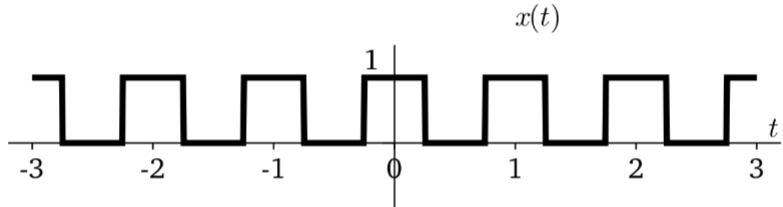
\includegraphics[scale=0.8]{W4_7.png}
\end{center}
Let's calculate the Fourier series for this.  First, we note that we only need to look at one period, so let's look from $t = -0.5$ to $0.5$, where the square wave starts at $0$ and transitions to $1$ at $t = -0.25$ and from $1$ back to $0$ at $t = 0.25$.  Let's define:
\[s(t) = \begin{cases} 0 & -0.5 \leq t < -0.25 \text{ and } 0.25 \leq t < 0.5 \\ 1 & -0.25 \leq t < 0.25\end{cases}\]
When we calculate the Fourier series, we should worry about two cases: when $k = 0$ and $k \neq 0$.  (Usually, if we just solve for when $k \neq 0$, we'll get an expression that is undefined for $k = 0$.  This is why we do both.)\\\\
For our square wave, we have that $T_0 = 1$.  When $k = 0$, 
\[c_k = \frac{1}{T_0} \int_{t_0}^{t_0 + T_0} f(t) e^{-jk\omega_0 t}\text{d}t\]
When $k \neq 0$,
\begin{align*}
    c_k &= \frac{1}{T_0} \int_{t_0}^{t_0 + T_0} f(t) e^{-jk\omega_0 t}\text{d}t\\
    &= \frac{1}{1} \int_{-0.5}^{0.5} s(t) \cdot e^{-jk\omega_0 t} \text{d}t\\
    &= \int_{-0.25}^{0.25} 1 \cdot e^{-jk\omega_0 t} \text{d}t\\
    &= -\frac{1}{jk\omega_0} e^{-jk\omega_0 t} \rvert_{t = -0.25}^{t = 0.25}\\
    &= -\frac{1}{jk\omega_0} \cdot \left[\left(\cos\left(k \cdot 2\pi \cdot \frac{1}{4}\right) - k \cdot \sin\left(k \cdot 2\pi \cdot \frac{1}{4}\right)\right)\right. \\
    &\hspace{2cm}- \left.\left(\cos\left( k \cdot 2\pi \cdot \frac{1}{4}\right) + j \cdot \sin\left(k \cdot 2\pi \cdot \frac{1}{4}\right)\right)\right]\\
    &= -\frac{1}{jk\cdot 2\pi} \left[ -2j \cdot \sin\left(\frac{k\pi}{2}\right)\right]\\
    &= \frac{\sin(k\pi / 2)}{k\pi}
\end{align*}

The term $\frac{\sin(\pi t)}{\pi t}$ occurs so frequently in signal processing that it has its own name:
\newcommand{\sinc}{\text{sinc}}
\[\sinc(t) \triangleq \frac{\sin(\pi t)}{\pi t}\]
The $\sinc$ function looks like:
\begin{center}
    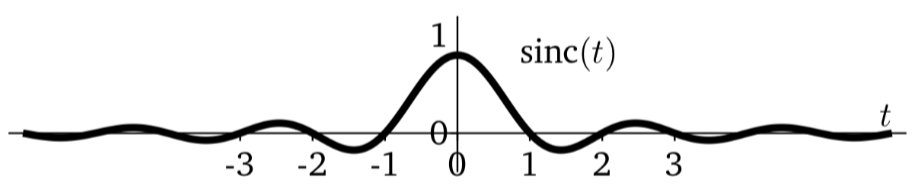
\includegraphics[scale=0.7]{W4_8.png}
\end{center}
(Note that some define $\sinc(t) = \sin(t) / t$.  We do NOT use this definition.)\\\\
Thus, we have that
\[c_k = \frac{1}{2} \sinc(k / 2)\]
Note that $\sinc(0) = 1$.

\pagebreak
\subsubsection*{Plotting the Square Wave Fourier Series}
Let's plot Fourier series fits for our square waves with one complex exponential frequency.
\begin{center}
    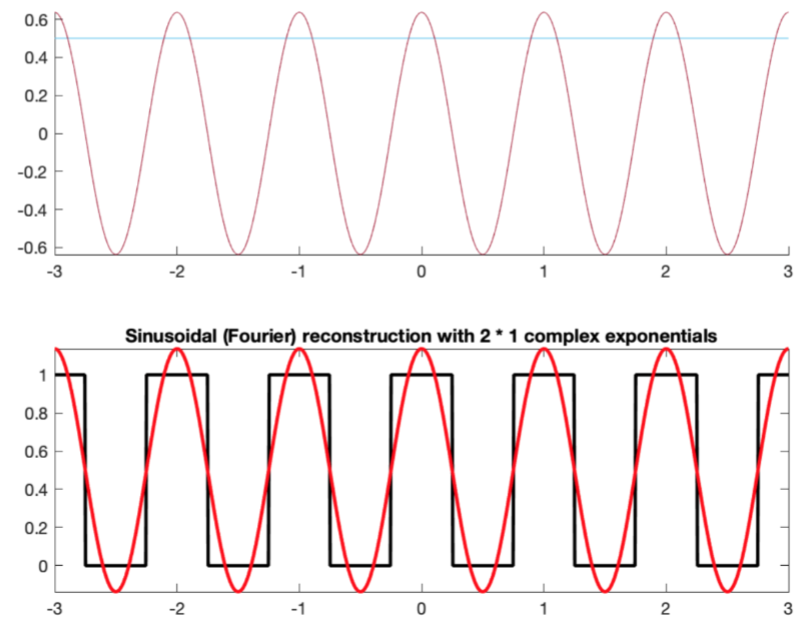
\includegraphics[scale=0.7]{W4_9.png}
\end{center}
Now, with three:
\begin{center}
    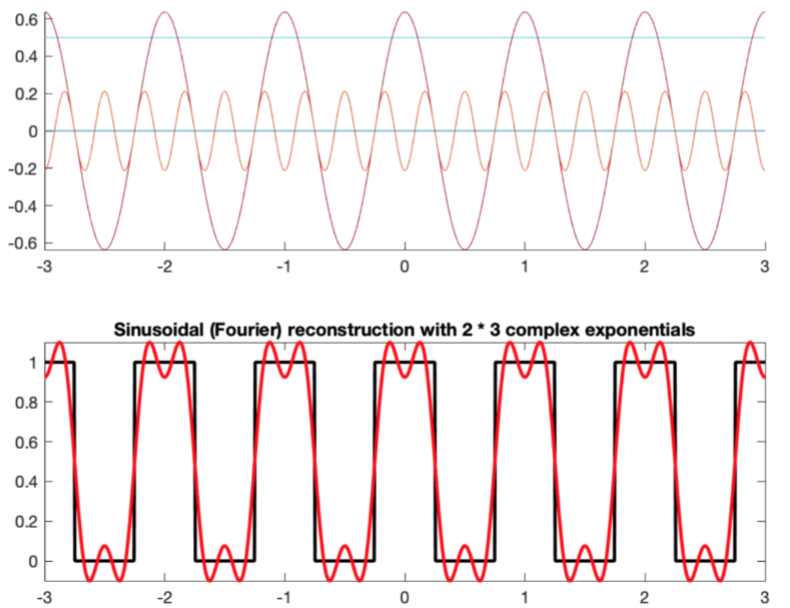
\includegraphics[scale=0.7]{W4_10.png}
\end{center}
\pagebreak
Now, with 10?
\begin{center}
    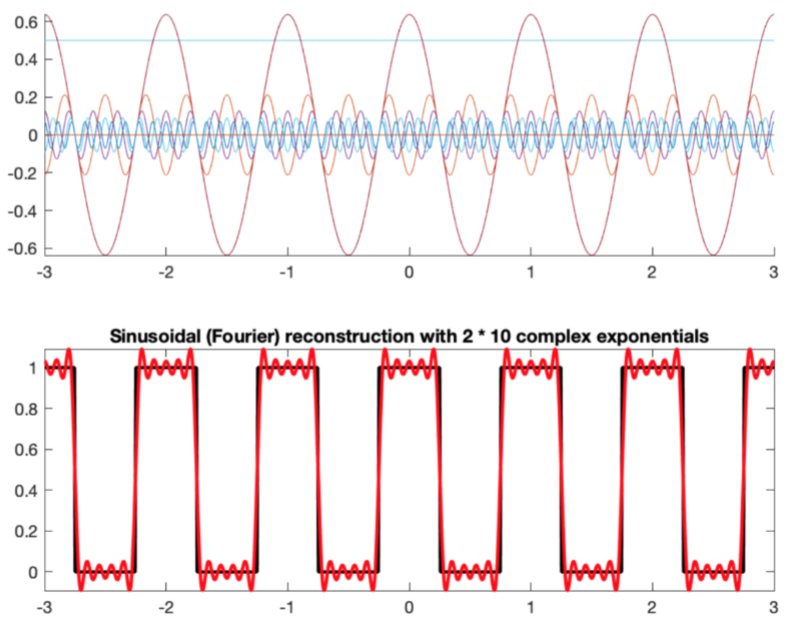
\includegraphics[scale=0.7]{W4_11.png}
\end{center}
And\dots with 100:
\begin{center}
    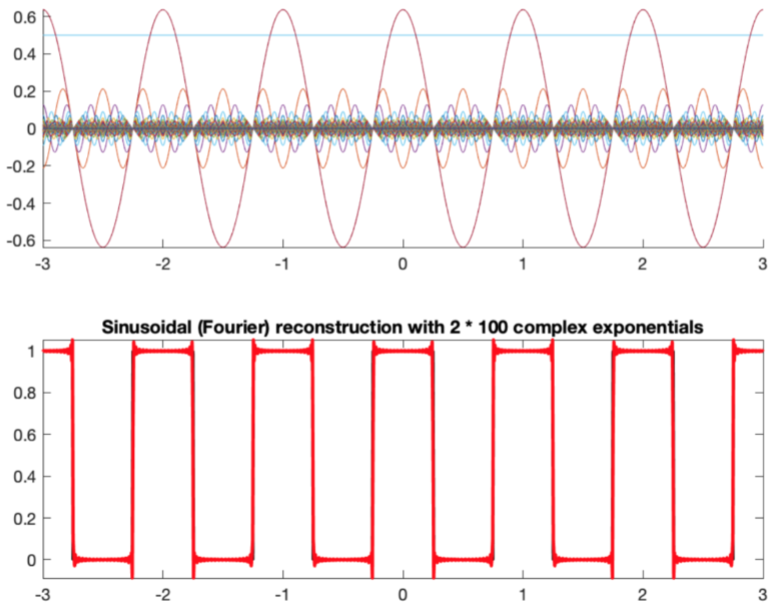
\includegraphics[scale=0.7]{W4_12.png}
\end{center}
\pagebreak
Do they converge?  Can we definitely say that for
\[c_k = \frac{1}{T_0} \int_{t_0}^{t_0 + T_0} f(t) e^{-jk\omega_0 t} \text{d}t\]
that
\[f(t) = \sum_{k = -\infty}^\infty c_k e^{jk\omega_t}\]
at every point in time $t$?\\\\
The answer is no.  If you notice our derivation, we only showed that this holds when $f(t)$ or its Fourier series representation are in an integral, i.e.,
\[\int_{t_0}^{t_0 + T_0} f(t) e^{-jn\omega_0 t} \text{d}t = \int_{t_0}^{t_0 + T_0} \left(\sum_{k = -\infty}^\infty c_k e^{jk\omega_0 t}\right) e^{-jn\omega_0 t}\text{d}t\]
What this means is that our Fourier series formula really only holds in the sense of the integral average over this period.  But it need not be the case that our Fourier series formula holds at exactly every single $t$.\\\\
\textbf{Fourier series does not equal $f(t)$ everywhere.}\\\\
As we can see, the Fourier series does not equal $f(t)$ everywhere.  However, it does a very reasonable job at fitting the square wave. There is work (we won't cover) on things we observe, like the "ringing" (called Gibbs effect) of the Fourier series at discontinuities. Interestingly, increasing the number of terms compresses the ringing but does not reduce its amplitude. You can see it's still present with $k = 100$ complex exponential frequencies in our square wave example.\\\\
There are \textit{Dirichlet} conditions that describe when $f$ can be approximated by a Fourier series. We won't talk about these in depth in class, but essentially, the signal should be "smooth" and "well-behaved" for a Fourier series approximation to be good.\\\\
In our square wave, there is no absolute for it using a Fourier series.

\subsection*{Sawtooth Signal}
The sawtooth signal is given by $f(t) = t \mod 1$.  It is plotted below:
\begin{center}
    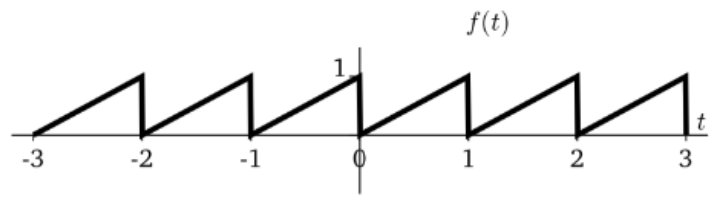
\includegraphics[scale=0.9]{W4_13.png}
\end{center}
This signal has a period of $T_0 = 1$.  Now, when $k = 0$,
\begin{align*}
    c_0 &= \int_0^1 te^0 \text{d}t\\
    &= \left.\frac{t^2}{2}\right|_0^1\\
    &= \frac{1}{2}
\end{align*}


\end{document}
